\documentclass[a4paper]{article}

\usepackage{fullpage} % Package to use full page
\usepackage{parskip} % Package to tweak paragraph skipping
\usepackage{tikz} % Package for drawing
\usepackage{amsmath}
\usepackage{hyperref}

\title{Circus Specification}
\author{Ashley J. Robinson}
\date{\today}

\begin{document}

\maketitle

\section{Introduction}

   \subsection{Acronyms} 
      \begin{table}[h]
         \centering
         \caption{Acronyms}
         \label{tab_acronyms}
         \begin{tabular}{|l|l|}
            \hline
            \textbf{Acronyms}    &  \textbf{Description}                         \\ \hline  
            CMD                  &  Command                                      \\ \hline
            ID                   &  Identity                                     \\ \hline
            IR                   &  Infra-Red                                    \\ \hline
            PW                   &  Parity Word                                  \\ \hline
            UART                 &  Universal Asynchronous Receiver-Transmitter  \\ \hline  
         \end{tabular}
\end{table}  


\section{Agent}

   \subsection{ID}
      \begin{itemize}
         \item Agents have hardware pin straps to configure IDs
         \item Agents have a valid ID range of 0x01 to 0xFE inclusive
         \item Agent ID = pin strap value + 1
      \end{itemize}
  

\section{Communications}
 
\begin{itemize}
   \item The communication scheme overview is shown in Figure~\ref{fig_communications}. 
\end{itemize}


\begin{figure}[h]
   \centering
   \label{fig_communications}
   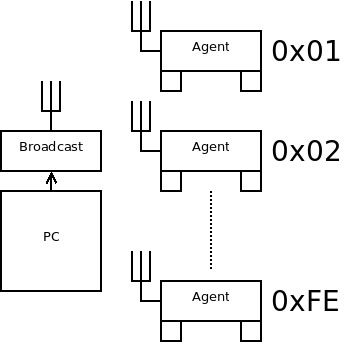
\includegraphics[width=6cm,keepaspectratio]{communications/communications.png} 
   \caption{Communication overview.}
\end{figure}
 
   \subsection{Receiver}
      \begin{itemize}
         \item The IR receiver will be connected to UART receiver of the microcontroller. 
         \item The receiver is initially in the \textbf{OFF} state. 
         \item The recover polls every 200ms for a carrier.
         \item The receiver must successfully find a carrier in two adjacent polls to switch the 
               receiver in to the \textbf{ON} state.
         \item Once in the \textbf{ON} state the receiver will constantly monitor the presence 
               of a carrier and return to the `\textbf{OFF} state when the carrier is lost. 
               This is 
      \end{itemize}

      \begin{figure}[h]
         \centering
         \label{fig_communications_time}
         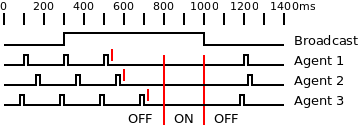
\includegraphics[width=10cm,keepaspectratio]{communications/communications_time.png} 
         \caption{Communication initiate timeout.}
      \end{figure}



\begin{itemize}
   \item    The agent receiver state machine is shown in Figure~\ref{fig_communications_sm}.
   \item    0xFF is invalid in both the \textbf{ID} and \textbf{CMD} states and will 
            push the state back to idle \textbf{ID} state. This can be used to reset the state machine
            as flushing with 0xFF will have no action.
   \item    Unmatching IDs will be stalled to allow \textbf{CMD} and \textbf{PW} to pass which may clash with valid \textbf{IDs}. 
   \item    Valid agents are shown in Table~\ref{tab_ids}.
   \item    Upon leaving the \textbf{ID} state an action must be reached before 50ms.
            An example of a completed and timed out transaction is shown in Figure~\ref{fig_communications_wave}.
   \item    The 
\end{itemize}

\begin{figure}[h]
   \centering
   \label{fig_communications_sm}
   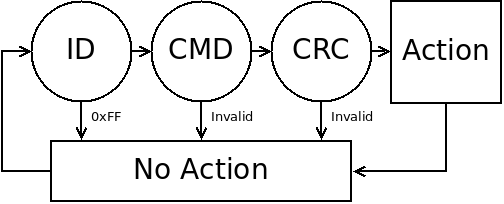
\includegraphics[width=8cm,keepaspectratio]{communications/communications_sm.png} 
   \caption{Communication state machine.}
\end{figure}

\begin{figure}[h]
   \centering
   \label{fig_communications_wave}
   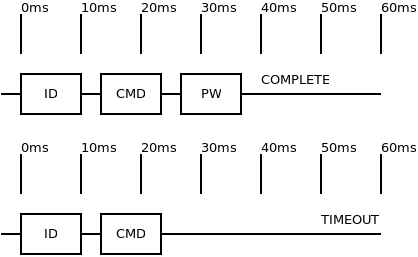
\includegraphics[width=8cm,keepaspectratio]{communications/communications_wave.png} 
   \caption{Communication message timeout.}
\end{figure}



\begin{table}[h]
   \centering
   \caption{Valid agent IDs.}
   \label{tab_ids}
   \begin{tabular}{|l|l|l|l|l|l|}
        \hline
        \textbf{ID}  &  \textbf{Description} \\ \hline  
         0x00        &  Issue the following command to all agents.\\ \hline  
         0x01..0xFE  &  Issue the following command to all agents with matching IDs.\\ \hline  
         0xFF        &  Resets the agent receiver state machine. \\ \hline  
   \end{tabular}
\end{table}




\end{document}
